\section{Theory}
\label{sec:theory}

Gamma-ray spectroscopy uses characteristic photon energies and intensities
to identify radionuclides and determine their activities. The following
sections outline gamma emission, photon interactions with matter, and signal
formation in a germanium detector.

\subsection{Gamma emission and activity}
\label{sec:gamma-emission}

Gamma radiation is emitted when an excited nucleus makes a transition to a
lower nuclear energy level. This process can be written schematically as
\begin{equation}
  \mathrm{X}^{*}\longrightarrow\mathrm{X}+\gamma,
  \label{eq:gamma-decay}
\end{equation}
where $\mathrm{X}^{*}$ denotes the excited nucleus.
Such excited states are often populated by a preceding radioactive decay.
The photon energy equals the difference between the two levels. 
The discrete nuclear levels therefore produce characteristic gamma lines,
which can be used to identify the emitting nuclide. For a single
radioactive nuclide, the activity $A$ follows the exponential decay law
\begin{equation}
  A(t)=A(t_0)\E^{-\lambda(t-t_0)}.
  \label{eq:activity}
\end{equation}
The decay constant $\lambda$ is related to the half-life by
\begin{equation}
  \lambda=\frac{\ln 2}{T_{1/2}}.
  \label{eq:decay-constant}
\end{equation}
Here $T_{1/2}$ is the half-life and $t_0$ the reference date.
Activity is measured in becquerel,
$\SI{1}{\becquerel}=1\,\mathrm{s}^{-1}$.
Each gamma line has its own emission probability $p_i$.
The photon emission rate of line $i$ is the source activity multiplied by $p_i$.


\subsection{Photon matter interactions}
\label{sec:photon-interactions}

Photons interact with matter through several mechanisms. In the \emph{photoelectric effect}, a photon is absorbed and an
atomic electron is emitted with kinetic energy approximately $E_\gamma-B$,
where $B$ is its binding energy. Photoelectric absorption is particularly important
at low photon energies and increases strongly with atomic number.

In \emph{Compton scattering}, a photon transfers part of its energy to an
electron and continues with a lower energy. Escape of the scattered photon
leaves only part of the incident energy in the detector. This process is
important at intermediate gamma energies and depends primarily on the
electron density. 

\emph{Pair production} becomes possible in the nuclear
field above $2m_ec^2\simeq\SI{1.022}{\mega\electronvolt}$: a photon converts
into an electron and a positron. After slowing down, the positron normally
annihilates into two photons of \SI{511}{\kilo\electronvolt} each.
Pair production becomes increasingly important at high energies. 
The relative contributions in germanium are illustrated in
Figure~\ref{fig:attenuation}.

\begin{figure}[!htb]
  \centering
  % Original image from ORTEC, Overview of Semiconductor Photon Detectors,
% Figure 3, page 1. Extracted directly from the source PDF without alteration.
% Source citation: ortec-photon-overview in references.bib.
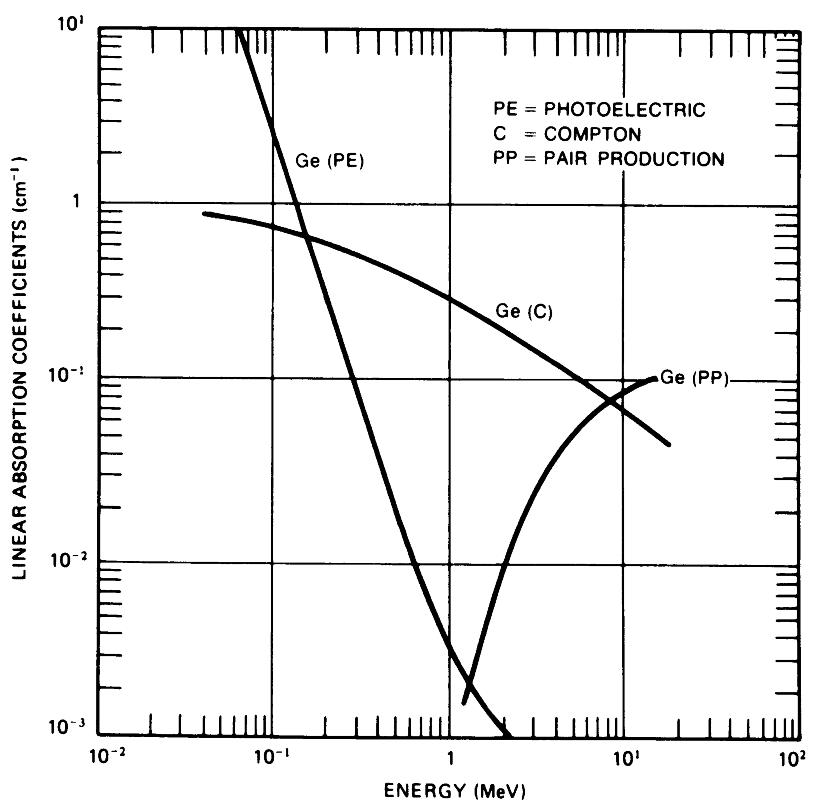
\includegraphics[width=0.72\textwidth]{figures/ortec_ge_attenuation.png}

  \caption{Linear attenuation coefficients of germanium as a function of
  photon energy for photoelectric absorption (PE), Compton scattering (C),
  and pair production (PP). Taken from Figure~3 in
  ORTEC~\cite{ortec-photon-overview}.}
  \label{fig:attenuation}
\end{figure}

\subsection{Attenuation and interaction probability}

For monoenergetic photons passing through a homogeneous material of thickness
$x$, the unscattered intensity follows
\begin{equation}
  I(x)=I_0\E^{-\mu x},
  \label{eq:attenuation}
\end{equation}
where $I_0$ is the incident intensity and $\mu$ the energy-dependent linear
attenuation coefficient. For a photon path of length $L$, the probability
of at least one interaction is
\begin{equation}
  P_{\mathrm{int}}=1-\E^{-\mu L}.
  \label{eq:interaction-probability}
\end{equation}
An interaction does not necessarily deposit the full photon energy, since
scattered photons can escape from the detector.

\subsection{Semiconductor detector and energy resolution}
\label{sec:semiconductor}

A germanium detector operates as a reverse-biased semiconductor diode.
The applied voltage widens the depletion region, which contains few mobile
charge carriers, and establishes an electric field. Energetic electrons
produced by photon interactions excite electrons from the valence band into
the conduction band, creating electron--hole pairs. The field drives electrons
and holes towards opposite contacts, producing a pulse whose height is
proportional to the deposited energy. Cooling suppresses leakage-current noise,
which results from thermal excitation of electrons across the band gap.
Figure~\ref{fig:detector-schematic} illustrates
the contact arrangement and
charge separation in a coaxial germanium detector.
An aluminium cover protects the germanium crystal.

\begin{figure}[!htb]
  \centering
  % Original longitudinal section, based on the geometry in the V18 manual.
% Requires TikZ and the arrows.meta library. Dimensions are schematic.
\begin{tikzpicture}[
  x=1cm,y=1cm,
  font=\small,
  >=Latex,
  leader/.style={draw=black!65,thin},
  carrier/.style={->,line width=0.8pt}
]
  % Protective cap, with a gap to the detector surface.
  \draw[gray!70,line width=2pt]
    (3.55,-0.05) -- (3.55,4.15) -- (9.25,4.15) -- (9.25,-0.05);

  % The depleted Ge volume surrounds the axial bore.
  \path[fill=blue!9,draw=blue!50!black,line width=0.6pt]
    (4.1,0) -- (4.1,3.6) -- (8.7,3.6) -- (8.7,0)
    -- (6.95,0) -- (6.95,2.45) -- (5.85,2.45) -- (5.85,0) -- cycle;

  % Outer Li-diffused contact and gold-coated bore contact.
  \draw[orange!85!black,line width=3pt]
    (4.1,0) -- (4.1,3.6) -- (8.7,3.6) -- (8.7,0);
  \draw[yellow!65!black,line width=2pt]
    (5.85,0) -- (5.85,2.45) -- (6.95,2.45) -- (6.95,0);

  \node[align=center,text=blue!50!black] at (6.4,3.05)
    {Depleted Ge\\active volume};
  \node[align=center,font=\footnotesize] at (6.4,1.1)
    {Axial\\bore};

  % A gamma creates carriers; the arrows show radial drift directions.
  \draw[->,blue!65!black,line width=0.9pt]
    (5.05,5.1) -- (5.05,1.58);
  \node[anchor=east,align=right] at (4.8,4.8)
    {Incident\\$\gamma$ photon};
  \fill[blue!65!black] (5.05,1.4) circle (1.4pt);
  \draw[carrier,blue!70!black] (4.99,1.4) -- (4.37,1.4);
  \draw[carrier,red!70!black] (5.11,1.4) -- (5.63,1.4);
  \node[blue!70!black,above] at (4.65,1.43) {$e^-$};
  \node[red!70!black,above] at (5.4,1.43) {$h^+$};
  \node[align=center,font=\footnotesize] at (4.99,0.55)
    {Charge\\separation};

  % Labels are outside the section, with no implied contact thickness.
  \draw[leader] (3.55,3.9) -- (2.9,4.05) -- (0.8,4.05);
  \node[anchor=south west,align=left] at (0.75,4.12)
    {Al protective\\cover};

  \draw[leader] (8.7,2.8) -- (9.6,3.15) -- (12.65,3.15);
  \node[anchor=south west,align=left] at (9.65,3.22)
    {Li-diffused outer contact};

  \draw[leader] (6.95,0.75) -- (9.6,0.2) -- (12.65,0.2);
  \node[anchor=south west,align=left] at (9.65,0.27)
    {Au-coated inner contact};

  % Reverse-bias voltage with contact connections, as in the manual.
  \draw[black!80] (8.7,0) -- (8.7,-0.9) -- (10.8,-0.9);
  \draw[black!80] (6.95,0) -- (6.95,-1.9) -- (10.8,-1.9);
  \draw[<->,black!80] (10.35,-0.98) -- (10.35,-1.82)
    node[midway,left] {$U$};
  \node[red!75!black,anchor=west] at (10.85,-0.9) {$+$};
  \node[blue!70!black,anchor=west] at (10.85,-1.9) {$-$};

\end{tikzpicture}

  \caption{Schematic coaxial Ge detector based on the
  manual~\cite{v18-manual}. The applied bias drives electrons and holes
  towards opposite contacts. Arrows indicate their drift directions.
  Not to scale.}
  \label{fig:detector-schematic}
\end{figure}

Even for identical deposited energies, the number of electron--hole pairs
fluctuates statistically, so the measured pulse heights are gaussian distributed around
a mean value. Electronic noise and variations in charge collection further
broaden this distribution. Its full width at
half maximum (FWHM) characterises the energy resolution: a smaller width
allows nearby gamma lines to be distinguished more clearly.

The full-energy detection efficiency $\varepsilon(E_i)$ is the probability
that a photon incident on the detector deposits its complete energy. For an
isotropically emitting source, it is given by
\begin{equation}
  \varepsilon(E_i)=\frac{N_i}{A\,t\,p_i\,\Omega/(4\pi)},
  \label{eq:full-energy-efficiency}
\end{equation}
where $N_i$ is the background-corrected peak area, $A$ the source activity,
$t$ the live time, $p_i$ the line emission probability, and $\Omega$ the solid
angle subtended by the detector as viewed from the source. The efficiency depends on
photon energy and detector geometry.

\subsection{Spectral features of a monochromatic gamma source}
\label{sec:compton-spectrum}

A monochromatic gamma source produces a full-energy peak and a Compton
continuum, illustrated in Figure~\ref{fig:spectrum-schematic}. The
full-energy peak represents complete energy deposition, either directly or
through successive interactions ending in absorption. The continuum arises
when a scattered photon escapes after transferring only part of its energy.

\begin{figure}[H]
  \centering
  % Original schematic: normalised energy, illustrative heights and widths.
% alpha = E_gamma/(m_e c^2) = 1.3, representative of the Cs-137 regime.
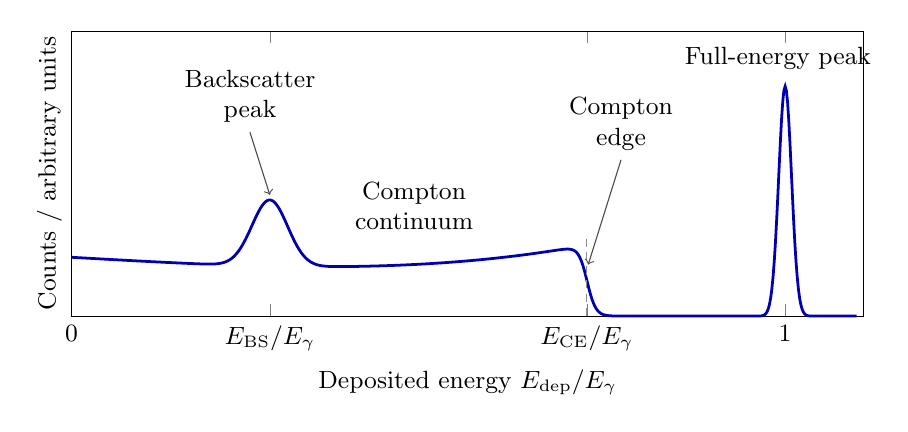
\begin{tikzpicture}
  \begin{axis}[
    width=0.96\textwidth,height=5.2cm,
    xmin=0,xmax=1.11,ymin=0,ymax=1.55,
    xlabel={Deposited energy $E_{\mathrm{dep}}/E_\gamma$},
    ylabel={Counts / arbitrary units},
    xtick={0,0.27778,0.72222,1},
    xticklabels={$0$,$E_{\mathrm{BS}}/E_\gamma$,$E_{\mathrm{CE}}/E_\gamma$,$1$},
    ytick=\empty,
    tick label style={font=\small},label style={font=\small},
    clip=false,
  ]
    % Smooth illustrative continuum and separate illustrative peaks.
    \addplot[blue!70!black,line width=1pt,domain=0:1.1,samples=650]
      {(0.32-0.22*x+0.60*x^3)/(1+exp((x-0.72222)/0.006))
        +0.36*exp(-0.5*((x-0.27778)/0.025)^2)
        +1.25*exp(-0.5*((x-1)/0.009)^2)};
    \draw[black!45,densely dashed] (axis cs:0.72222,0) -- (axis cs:0.72222,0.45);
    \draw[->,black!70] (axis cs:0.25,1.0) -- (axis cs:0.27778,0.66);
    \node[anchor=south,align=center,font=\small] at (axis cs:0.25,1.0)
      {Backscatter\\peak};
    \node[align=center,font=\small] at (axis cs:0.48,0.60)
      {Compton\\continuum};
    \draw[->,black!70] (axis cs:0.77,0.85) -- (axis cs:0.724,0.28);
    \node[anchor=south,align=center,font=\small] at (axis cs:0.77,0.85)
      {Compton\\edge};
    \node[anchor=south,align=center,font=\small] at (axis cs:0.99,1.29)
      {Full-energy peak};
  \end{axis}
\end{tikzpicture}

  \caption{Schematic gamma spectrum showing the full-energy peak, Compton
  continuum, Compton edge and backscatter peak. Relative heights and widths
  are illustrative.}
  \label{fig:spectrum-schematic}
\end{figure}

In Compton scattering from a free electron initially at rest, a photon with
incident energy $E_\gamma$ has the scattered energy $E'_\gamma$ given by
\begin{equation}
  E'_\gamma=\frac{E_\gamma}{1+\alpha(1-\cos\theta)},
  \label{eq:compton-energy}
\end{equation}
with
\begin{equation}
  \alpha=\frac{E_\gamma}{m_ec^2},
  \label{eq:compton-alpha}
\end{equation}
where $\theta$ is the scattering angle and $m_ec^2$ the electron rest energy.
The electron receives the difference between the incident and scattered
photon energies. The differential cross section for Compton scattering
is described by the Klein--Nishina formula
\begin{equation}
  \frac{\dif{\sigma}}{\dif{\Omega}}
    =\frac{r_e^2}{2}\left(\frac{E'_\gamma}{E_\gamma}\right)^2
    \left(\frac{E'_\gamma}{E_\gamma}
    +\frac{E_\gamma}{E'_\gamma}-\sin^2\theta\right),
  \label{eq:klein-nishina}
\end{equation}
where $r_e$ is the classical electron radius.

The maximum energy transfer at $\theta=\pi$ defines the Compton edge.
Photons scattered backwards in surrounding material and then absorbed in
the detector produce the backscatter peak. Their energies are
\begin{align}
  E_{\mathrm{CE}}&=E_\gamma\frac{2\alpha}{1+2\alpha},
  \label{eq:compton-features} \\
  E_{\mathrm{BS}}&=\frac{E_\gamma}{1+2\alpha}.
  \label{eq:backscatter-energy}
\end{align}
For a Gaussian full-energy peak, the full width at one tenth of the maximum
(FWTM) and the FWHM satisfy
\begin{equation}
  \frac{\mathrm{FWTM}}{\mathrm{FWHM}}
    =\sqrt{\frac{\ln10}{\ln2}}\simeq1.823.
  \label{eq:gaussian-width-ratio}
\end{equation}
Their measured ratio therefore tests the Gaussian peak shape.

\newpage